\documentclass[10pt,conference]{IEEEtran}
\IEEEoverridecommandlockouts
% The preceding line is only needed to identify funding in the first footnote. If that is unneeded, please comment it out.
\usepackage{cite}
\usepackage{amsmath,amssymb,amsfonts}
\usepackage{algorithmic}
\usepackage{graphicx}
\usepackage{textcomp}
\usepackage{xcolor}
\usepackage{subfig}
\usepackage{listings}
\lstset{numbers=left,stepnumber=1,basicstyle=\footnotesize\ttfamily}
\def\BibTeX{{\rm B\kern-.05em{\sc i\kern-.025em b}\kern-.08em
T\kern-.1667em\lower.7ex\hbox{E}\kern-.125emX}}
\def\code#1{\texttt{#1}}
\begin{document}

\title{A Second Look at the Dynamics of the JavaScript Package Ecosystem\\}

\author{\IEEEauthorblockN{Kevin de Haan, Gregory Neagu, Frederic Sauve-Hoover, Abram Hindle}
  \IEEEauthorblockA{\textit{Department of Computing Science} \\
    \textit{University of Alberta}\\
    Edmonton, Canada\\
  Email: \{kdehaan,neagu,rsauveho,abram.hindle\}@ualberta.ca}
}

\maketitle

% Footnote should maybe be a full source, or just one link
\begin{abstract}
  In recent years, the tools and packages most commonly involved with JavaScript development have evolved rapidly.
  Newer packages such as Angular and React have experienced a marked increase in popularity among developers, while frameworks such as jQuery
  have begun to phase out.\footnote{\label{adoption}https://insights.stackoverflow.com/survey/2016\#technology-most-popular-technologies, 
    https://insights.stackoverflow.com/survey/2017\#technology-\_-frameworks-libraries-and-other-technologies, 
  https://insights.stackoverflow.com/survey/2018\#technology-\_-frameworks-libraries-and-tools}
  For this reason we take a second look at a 2016 paper by Wittern, Suter and Rajagopalan \cite{Wittern:2016} 
  to see what aspects of the JavaScript package ecosystem have changed, and if previously observed trends have remained constant.
  In the original paper the authors use the \emph{node package manager} (\code{npm}) to gain 
  insight into the JavaScript ecosystem as a whole, and data from projects publicly hosted on 
  \code{GitHub} to observe an alternative measure of popularity. We adhere to the same methods of analysis, 
  and extend the data to capture more recent information up to April 1\textsuperscript{st} 2019.
  Ultimately, this second look aims to discover if recent years have had any significant effects on 
  ecosystem-wide trends, and provide developers with further insight into how packages are used and evolve.
\end{abstract}


\begin{IEEEkeywords}
  JavaScript; Node.js; node package manager; software ecosystem analysis
\end{IEEEkeywords}


\section{Introduction}
Software ecosystems are environments that form as projects develop in parallel,
becoming interconnected as contexts and dependencies span companies and communities \cite{LUNGU2010264}. 
Research on these systems has increased rapidly in the recent past \cite{Manikas:2017}, investigating
their characteristics and behaviour as they develop \cite{Manikas:2013}. Understanding how software
ecosystems evolve is important from both a software as well as a business standpoint\cite{Messerschmitt},
and is valuable for informing developers how technologies are used over time \cite{Serebrenik:2015}. 
An understanding of software ecosystems can inform decisions on when to adopt frameworks and how long
to support them, as well as provide insight into how changes to software propagate throughout the community \cite{Wittern:2016}.
Additionally, determining the characteristics of software ecosystems 
can help clarify why some frameworks flourish while others fail, and guide 
developers in the creation of new tools\cite{Serebrenik:2015}. Furthermore, 
because software projects are overwhelmingly a collaborative effort, a complete
understanding of a single project often requires knowledge of the ecosystem supporting it\cite{Blincoe:2015}.


This paper is a replication of \emph{A Look at the Dynamics of the JavaScript Package Ecosystem}\cite{Wittern:2016} 
that performs extensive analysis of the \emph{node package manager} (\code{npm}) ecosystem. 
\code{npm} provides a set of open source tools that allow developers to 
describe packages for \code{Node.js}, an asynchronous JavaScript runtime environment 
designed for network applications\footnote{https://nodejs.org/en/about/}.
The services provided by \code{npm} include a command line interface for maintaining 
\code{package.json} files, the primary method to describe package metadata such as the name,
description, version, and dependencies of a given package. \code{npm} also allows 
developers to publish their packages to a public registry, permitting anyone 
to download and use their software. Packages hosted on \code{npm} will often depend on other \code{npm}
packages, forming an elaborate JavaScript package ecosystem.
Since the publishing of the original paper, the usage and scale of \code{npm} has only grown,
and now hosts more than three times as many packages (over 750,000 as of April 1\textsuperscript{st} 2019) 
and handles over ten times as many weekly package downloads (now over ten billion per week).
Additionally, the major frameworks used in JavaScript development have undergone a 
rapid transformation as packages such as Angular and React are adopted\footnotemark{\ref{adoption}}.
The core contributions we make are as follows:
\begin{itemize}
  \item We replicate and verify the results found in the original paper for the 
    window of October 1\textsuperscript{st} 2010 to September 1\textsuperscript{st} 2015.
  \item We extend the analysis to the time period of September 2\textsuperscript{nd} 
    2015 to April 1\textsuperscript{st} 2019, and evaluate whether patterns and trends 
    noted in the original paper are still observable.
  \item We investigate whether the continued evolution of the JavaScript package 
    ecosystem has affected the relationships between various measures of package popularity.
  \item We determine if the ongoing maturation of the \code{npm} ecosystem has 
    resulted in tangible changes to version numbering or adoption practices.
\end{itemize}


\section{Data Collection}
% CHECK IF THE NUMBERS ARE RIGHT
The window of data analyzed within this paper is October 1\textsuperscript{st} 2010 (as in the original paper) to April 1\textsuperscript{st} 2019.
We collected from three publicly available data sets. Two of these, the \code{npm} registry and the \code{GitHub} repository platform, are from the same source as in the original paper.
To find repositories relying on \code{npm}, we used the Google BigQuery \code{github\_repos} data set, updated weekly\footnote{https://github.com/fhoffa/analyzing\_github/}.
By using this set we are able to analyze \code{GitHub} data without being constrained to the currently available window provided by the GHTorrent project\cite{Gousi13}.
The final data set encompasses 797,940 packages and \textbf{\#VALUE} applications.

\subsection{Package Metadata}

\begin{lstlisting}[caption={A mock \code{npm} package.json. Some fields omitted for brevity.},captionpos=b,
  label=samplePkg, frame=single, firstline=1]
{
  "name": "Lorem Ipsum",
  "version": "0.9.3",
  "maintainers": [
      {"name": "Dolor Sit",
      "email": "dolorsit@amet.org"}
  ],
  "repository": {
      "type": "git",
      "url": "https://github.com/lor/em"
  },
  "main" : "loremipsum.js",
  "keywords": ["Web", "REST"],
  "dependencies": {
      "Adipiscing": "~1.7.0",
      "Elit": "5.1.x"
  },
  "devDependencies": {
      "Sed": "0.9.0",
      "Do": ">=1.3.5 <4.0.0" 
  }
}
\end{lstlisting}

\begin{lstlisting}[caption={A mock simplified \code{npm} metadata file.},captionpos=b,
  label=sampleSimpleMetadata, frame=single, firstline=1][t]
{
  "name": "Lorem Ipsum",
  "versions": {
    "1.0.4": {
      "dependencies": {
        "Adipiscing": "~1.7.0",
        "Elit": "5.1.x"
      },
      "devDependencies": {
        "Sed": "0.9.0",
        "Do": ">=1.3.5 <4.0.0"
      }
    },
    "1.0.5": {
      "dependencies": {
        "Adipiscing": "~1.7.0",
      },
      "devDependencies": {
        "Do": ">=1.3.5 <4.0.0"
      }
    },
    "time": {
      "1.0.4": "2017-09-25T06:39:20.596Z",
      "1.0.5": "2018-05-22T08:35:40.227Z",
      "created": "2015-05-18T03:52:55.192Z"
    }
  }
}
\end{lstlisting}

Metadata for every package is available on the \code{npm} registry\footnote{https://registry.npmjs.org/packageName}. 
This metadata is a JSON file containing some info on licensing, documentation links, maintainers, and crucially for 
our purposes a log of each version of the package since it's creation, labelled using semantic versioning \cite{preston-werner},
and a time field containing the timestamp for each version. Each version in the version field contains various bits of 
version specific information such as authors, maintainers, license used, bugs, and a list of dependencies for that specific
version.\\

We obtained the list of all \code{npm} package names from the \code{npm} registry skimdb\footnote{https://skimdb.npmjs.com/registry/\_all\_docs}, and then %TODO fix this footnote, underscores are cursed
downloaded this metadata for all 797,940 packages on the \code{npm} registry, having found the names of all packages using the npm registry skimdb
, which we then converted to a somewhat simplified form as in Listing \ref{sampleSimpleMetadata} with just version and dependency information as this is all
we care about for this study. There are two kinds of dependencies in the metadata files, a list of runtime dependencies and $devDependencies$ used in testing and development.\\

We gathered some information on download counts for \code{npm} packages from the npmjs API\footnote{https://api.npmjs.org/downloads/range/2010-01-01:2019-04-01/packageName} 
however we found that the npmjs API seems to no longer have any data on download counts before October 1 2017, and so were unable to collect
historic download counts for \code{npm} as a whole or any specific packages.\\

\subsection{Applications using \code{npm} Packages}

To collect our data for package usage in public projects, 
we turned to the Google BigQuery \code{github\_repos} data 
set\footnote{https://bigquery.cloud.google.com/dataset/bigquery-public-dat:github\_repos}.
From this data, we skimmed all projects and pulled those 
written in JavaScript, resulting in an initial total of 9,017,221 
repositories. Simply being written in JavaScript is not enough to detect
\code{npm} usage, so to find repositories using \code{npm} packages
we looked for projects that contained a \code{package.json} 
file. After confirming that the formatting of the file matched the \code{npm}
standard, we are able to confidently say that any remaining packages are 
using \code{npm} packages. With this criteria, we then compiled a list 
of [100,000 for now] project 
repositories from GitHub, a volume that we felt is likely to be an 
appropriate representation of all such public projects.
Using the \code{GitHub} platform API and the list of valid repository names 
from before, we cloned the GitHub repository for each project. With
this, we were then able to determine the date and time of every 
commit of the project, as well as the list of included \code{npm} packages
at the time of commit, as listed in every historic version of 
\code{package.json}, providing us with the \code{npm} packages used by that repository
at any given time in the project's history. The results showed that on average a repository 
had 37.9 commits as well as [STATS HERE]. Ultimately, of the 9,017,221 
public \code{GitHub} projects written in JavaScript and the [NUMBER] of repositories
using \code{npm} packages, we randomly selected [NUMBER] repositories as
a representative data set for the analysis.


\section{Ecosystem Evolution}

\begin{figure}
  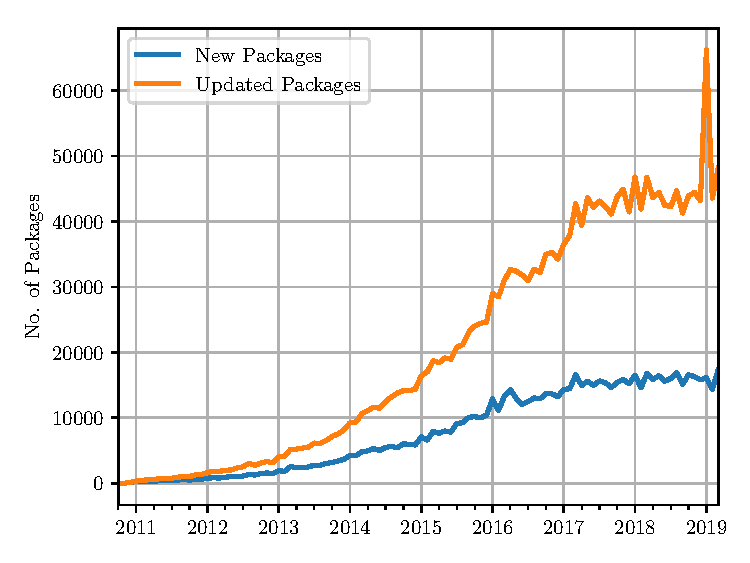
\includegraphics[width=0.5\textwidth]{figures/new_vs_updates_by_month.pdf}
  \caption{Packages updated and packages created per month. Multiple updates per month are
  only counted once.}
  \label{npmGrowth}
\end{figure}

Created in 2009, \code{npm} has grown
rapidly in popularity and scope over the last ten years, and 
as of the original paper showed no signs of slowing down \cite{Wittern:2016}.
We investigate the state of the \code{npm} ecosystem
since September 1\textsuperscript{st} 2015, and look for any signs of deterioration in 
the health of the ecosystem. Periods of stagnating growth would suggest
that developer interest is waning, while steady activity would 
indicate that the ecosystem as a whole is healthy and will continue to
evolve. To search for these potential indicators in the \code{npm} package environment,
we investigate the number of packages created and updated over time, as well
as system-wide trends of dependencies within packages. In Figure \ref{npmGrowth},
we can observe that while \code{npm} is still growing, the speed at which new packages
are created has slowed from an exponential to a linear rate. Some other things of note 
include an observable spike in package creation and updates around March 2016, the month 
when developer Azer Ko\c{c}ulu removed his 273 packages (including the popular package 
\code{left-pad}) from \code{npm} and in doing so affected some packages such as 
\code{babel} and \code{atom}, and therefore a significant fraction of \emph{all} 
\code{Node.js} projects\footnote{https://blog.npmjs.org/post/141577284765/kik-left-pad-and-npm}.
There is also a significant spike in package updates observed in the month of January 2019, caused 
by some source currently unknown to the authors [TRY TO FIGURE THIS ONE OUT].
[ADD CONCAVITY DATA]. Figure 2 [CURRENTLY MISSING][MORE DATA COMMENTARY].



To better visualize the status of inter-package dependencies, we constructed
a directed dependency graph using dependants as out-degrees and
dependencies as in-degrees. Based on this graph, Figure \ref{outDegree}
displays the percentage of packages with various amounts of dependencies. 
[MIGHT NEED TO CHANGE BASED ON DATA: While the average number of dependencies 
of packages continues to increase, the percentage of packages with zero 
to three dependencies has actually increased since the end of the original paper's
reporting period \cite{Wittern:2016}. This suggests some changes to developer 
behaviour, likely either as a deliberate effort by programmers seeking to avoid the perils of 
complicated dependency trees \cite{Kikas:2017}, or as a natural result of the ever-changing
ways in which JavaScript is used for project development. [ADD EXACT VALUES]

In addition to the number of external dependencies per package, 
we investigate how packages support dependants. The original paper 
discovered that the majority of in degrees are concentrated among a core 
minority of packages, with the majority of packages having no dependants,
a discovery that has also been observed in other software ecosystems such
as Linux and MySQL \cite{Myers:2003}. In our updated data, we discover 
that not only have these aspects held true, but the concentration of 
dependencies has actually increased. As of April 1\textsuperscript{st} 2019, [NUMBER]\% of packages
had zero dependants, up from [NUMBER]\% in 2015. Meanwhile, only \%[NUMBER] of packages
had 6 or more dependants, down from \%[NUMBER] in September 2015. It is again interesting to note
that the current trend of increasing concentration appears to have begun shortly after the end of window in the original
paper \cite{Wittern:2016}.

\begin{figure}
  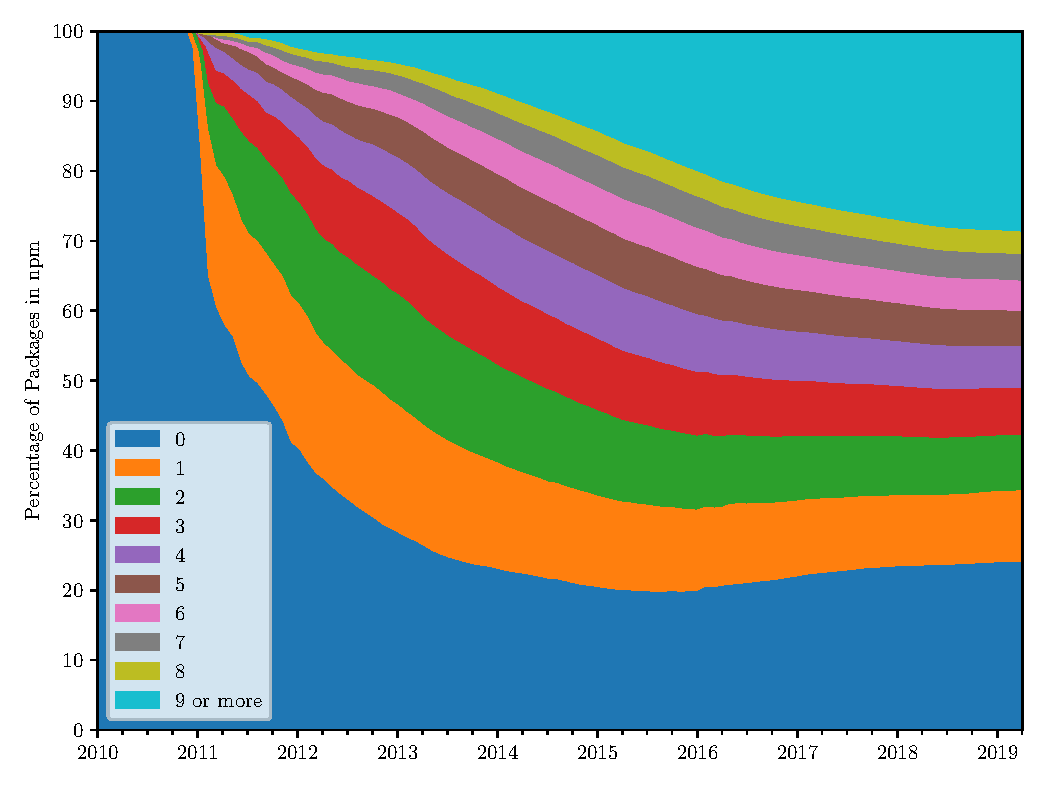
\includegraphics[width=0.5\textwidth]{figures/npm_deps_monthly_out_degree.pdf}
  \caption{\code{npm} packages by their number of dependencies on other packages}
  \label{outDegree}
\end{figure}

\begin{figure}
  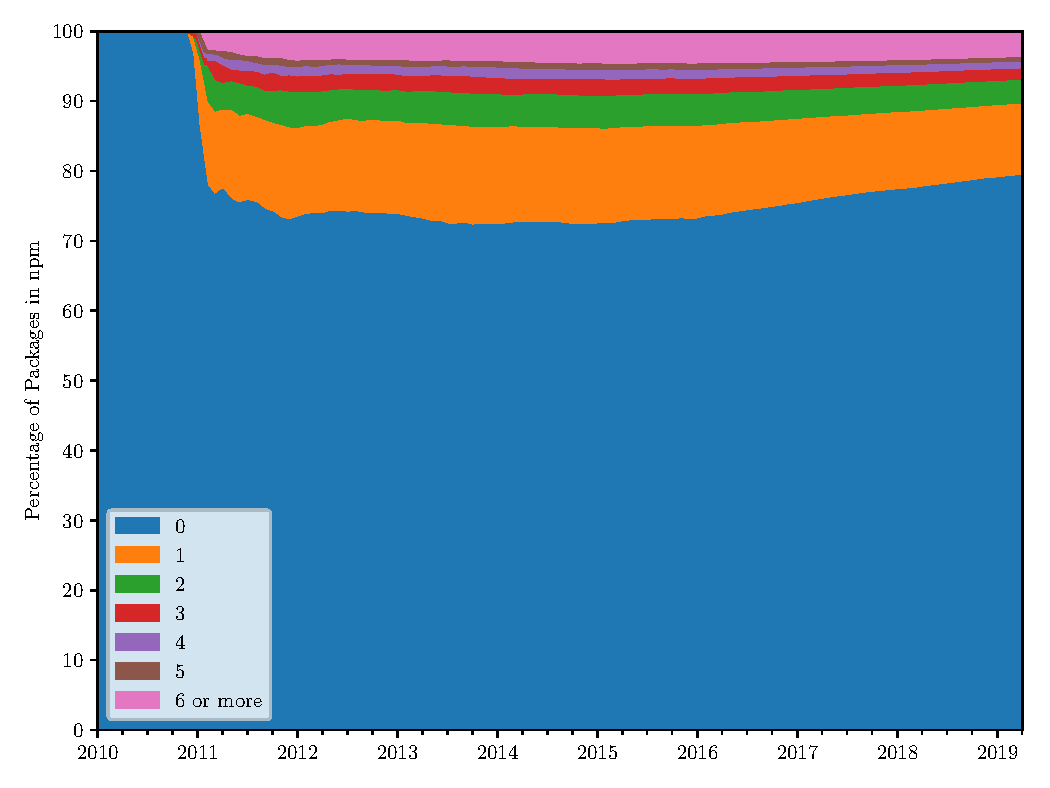
\includegraphics[width=0.5\textwidth]{figures/npm_deps_monthly_in_degree.pdf}
  \caption{\code{npm} packages by the number of other packages depending on them}
  \label{inDegree}
\end{figure}

\begin{figure}
  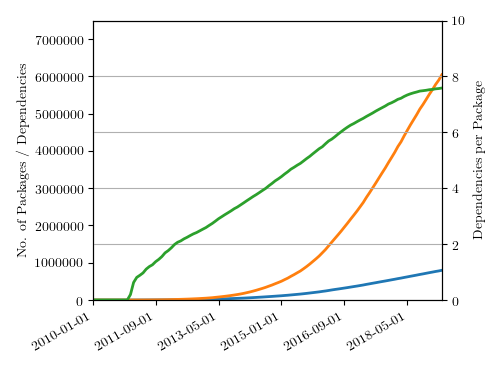
\includegraphics[width=1\linewidth]{figures/packages_vs_dependencies.png}
  \caption{axis \textbf{y1} shows growth in number of packages in npm (blue line), and the number of dependencies (orange line), 
  with axis \textbf{y2} showing average number of dependencies per package (green line)}
  \label{packVSDependencies}
\end{figure}

\begin{figure}
  % TODO NOTE THAT THIS HAS LOWER NUMBERS THAN THE ORIGINAL PAPER DUE TO MONTHLY PAGERANKS
  \begin{tabular}{c|c|c|c}
    Year & Top 10 & Top 100 & Top 250 \\
    \hline
    2010 & 13 & 103 & 253\\
    2011 & 25 & 297 & 701\\
    2012 & 6 & 46 & 136\\
    2013 & 3 & 38 & 114\\
    2014 & 1 & 40 & 96\\
    2015 & 4 & 38 & 86\\
    2016 & 4 & 29 & 62\\
    2017 & 0 & 12 & 48\\
    2018 & 0 & 15 & 31\\
    2019 & 0 & 4 & 12\\
  \end{tabular}
  \caption{Number of packages entering top \code{npm} ranks for the first time}
  \label{numEnteringTop}
\end{figure}

\section{Package Popularity}

As in the original paper we analyzed popularity of \code{npm} packages using three major measures
\begin{enumerate}
  \item The \textbf{\code{npm} rank} is calculated using the PageRank\cite{brin1998anatomy} of an \code{npm} package within a dependency graph that we built using the
    package metadata as described in Section \ref{Package Metadata}. PageRank is calculated for every package using a damping factor of 0.85 
    and stopping iterations once the cumulative change in values of vertices went below $10^{-6}$. We then order all packages by their PageRank to determine the
    \code{npm} rank, an relative ranking of packge popularity with 1 being the most popular.
  \item \textbf{download rank}
\end{enumerate}


\subsection{Relationships between Measures}
[NEEDS MORE DATA]

\subsection{Distinct Package Types}
[NEEDS MORE DATA]

\subsection{Popularity Over Time}
[NEEDS MORE DATA]

\subsubsection{Identifying Top Packages}
[NEEDS MORE DATA]

\begin{figure}
  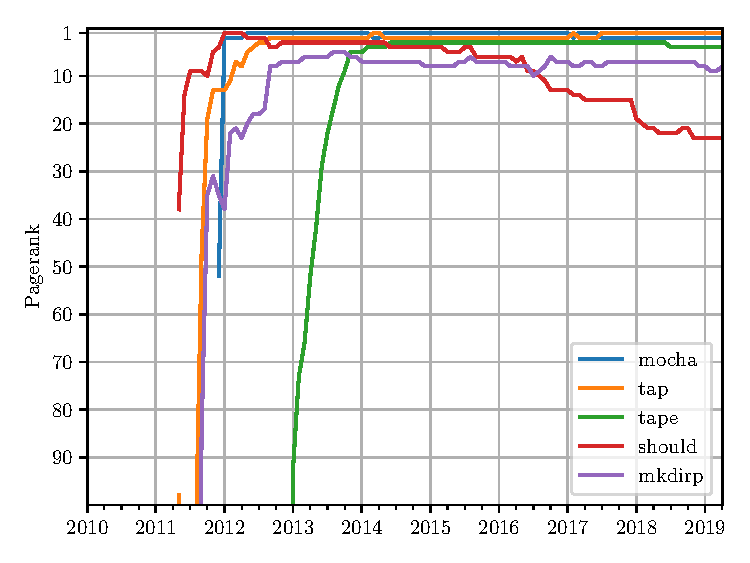
\includegraphics[width=0.5\textwidth]{figures/geo_mean_highest_pagerank.pdf}
  \caption{\code{npm} rank (PageRank) of the five packages with the lowest overall geometric mean}
  \label{topFive}
\end{figure}


\subsubsection{Popular Package Dynamics}
[NEEDS MORE DATA]

\begin{figure*}
  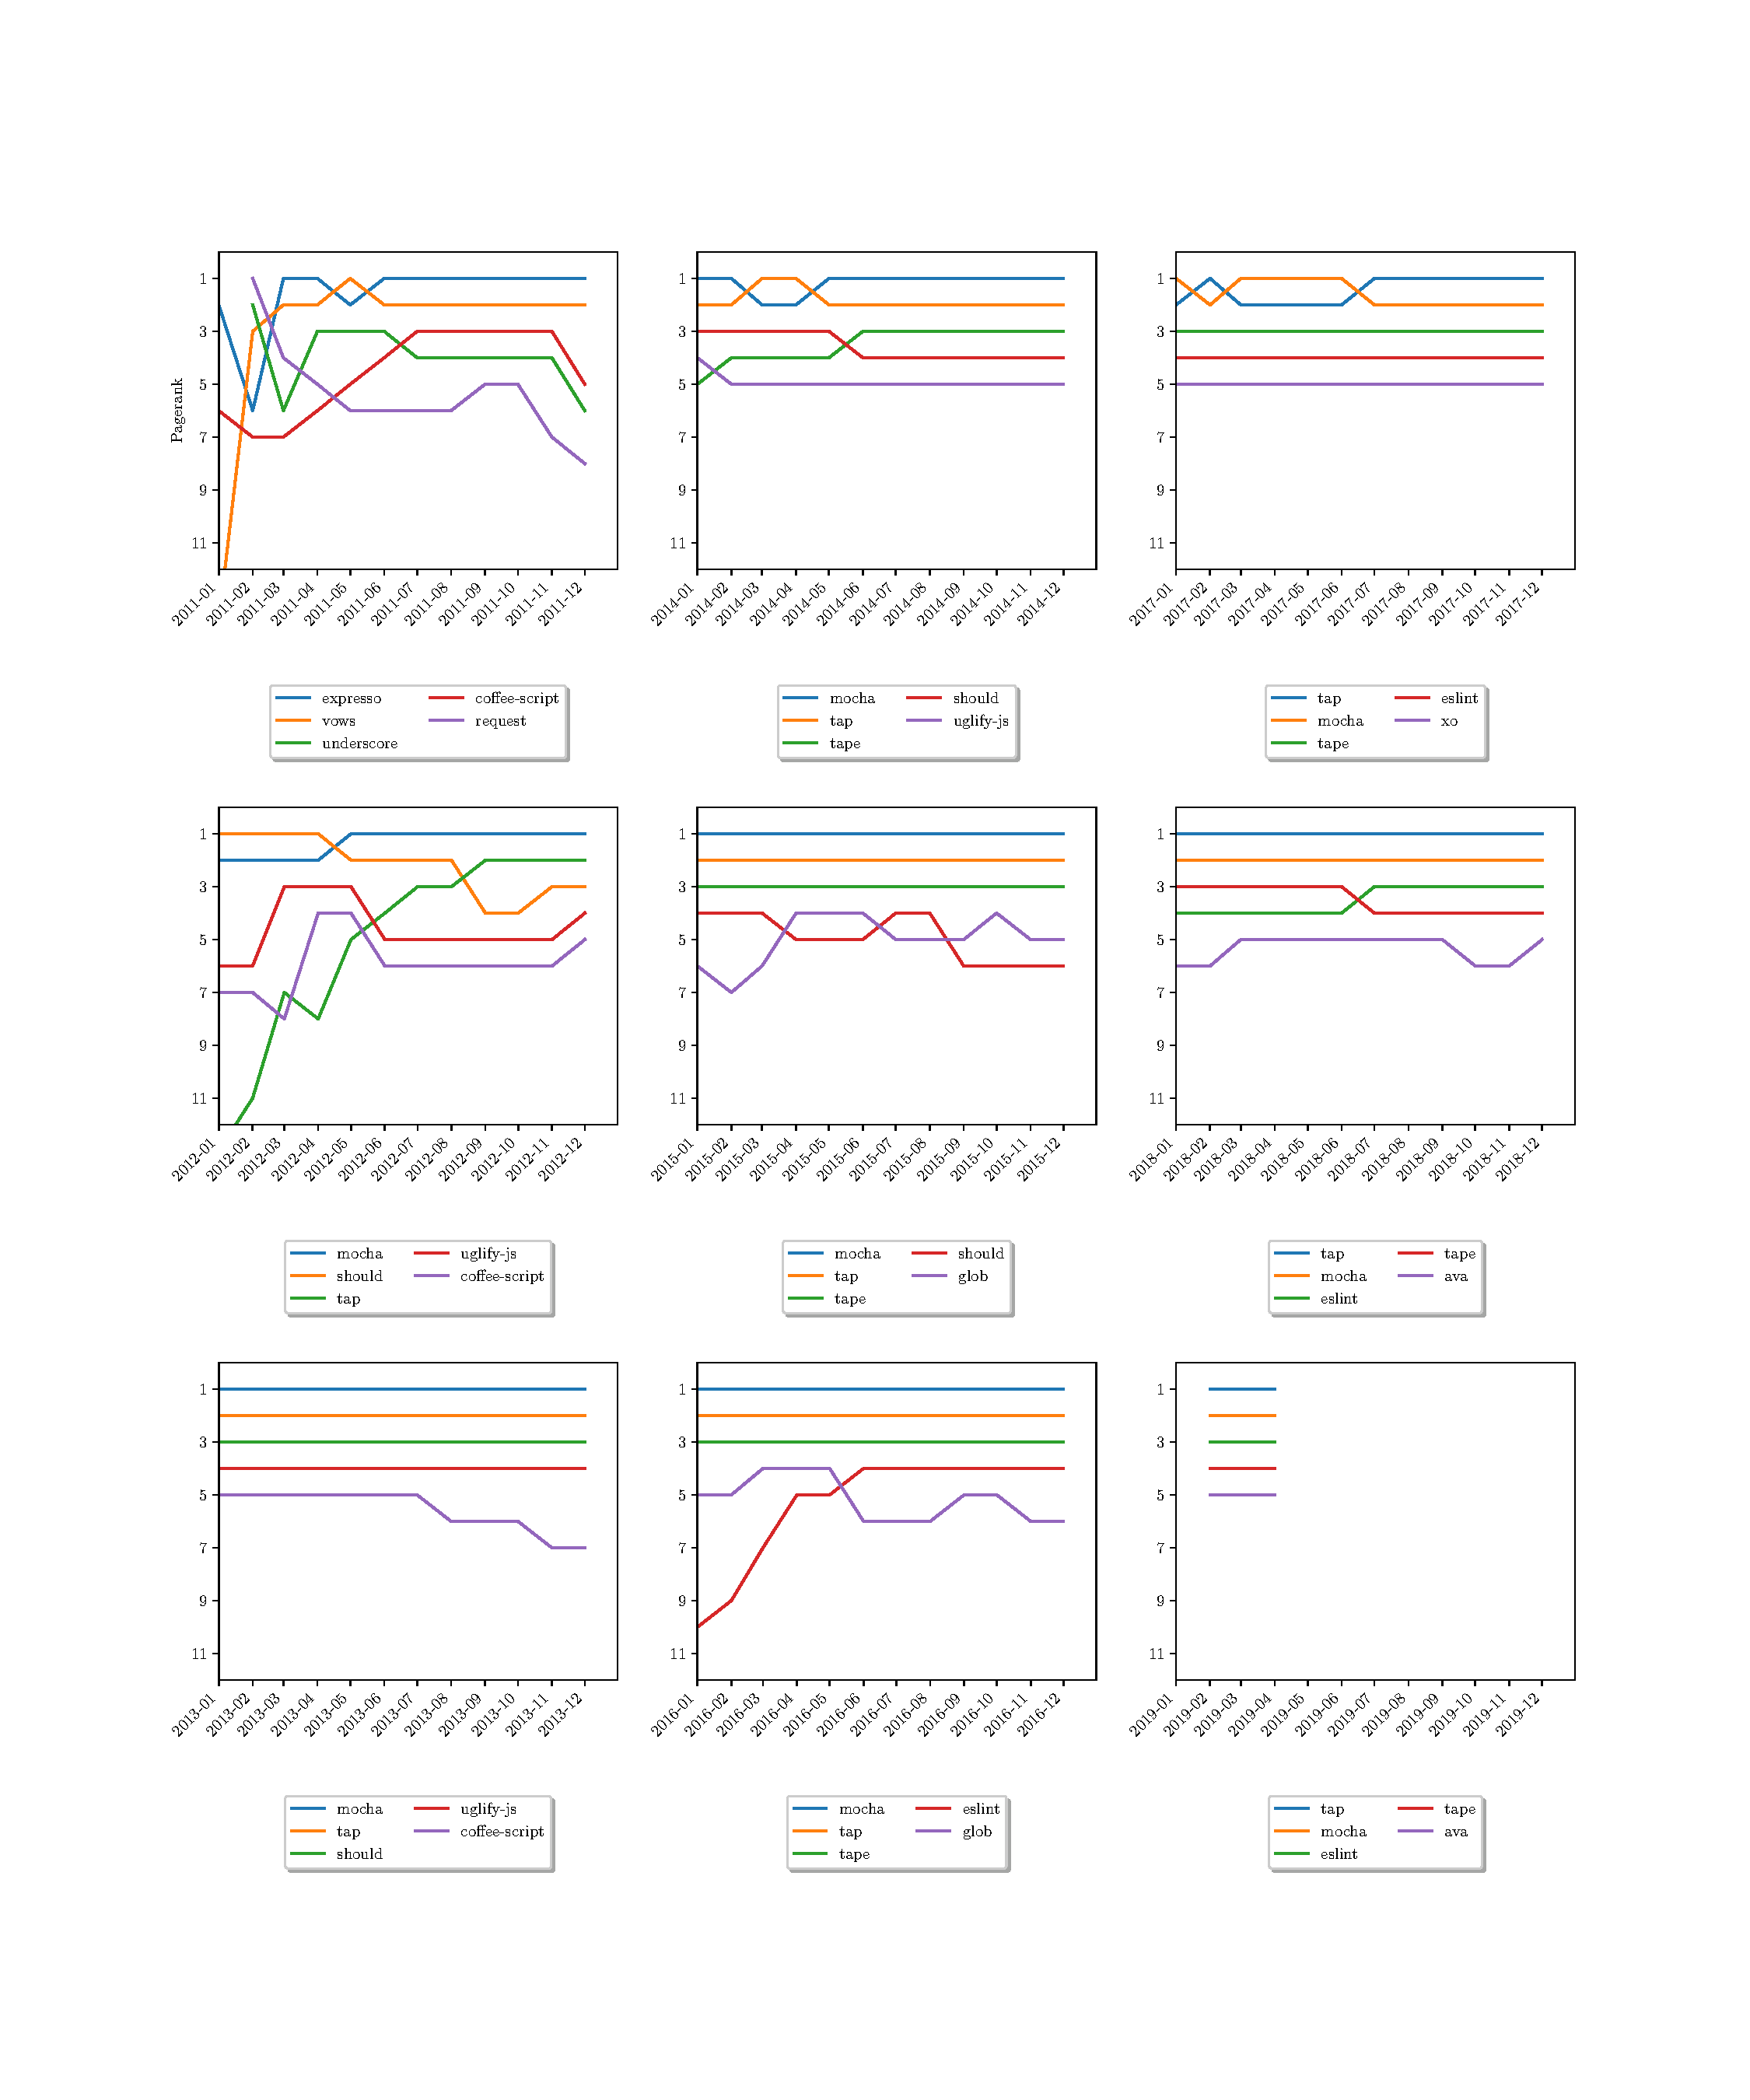
\includegraphics[width=1\textwidth]{figures/highest_ranked.pdf}
  \caption{\code{npm} rank (PageRank) of the five packages each year with the lowest geometric}
  \label{ranksByYear}
\end{figure*}

\subsubsection{Comparing Popularities}
[NEEDS MORE DATA]

\begin{figure}
  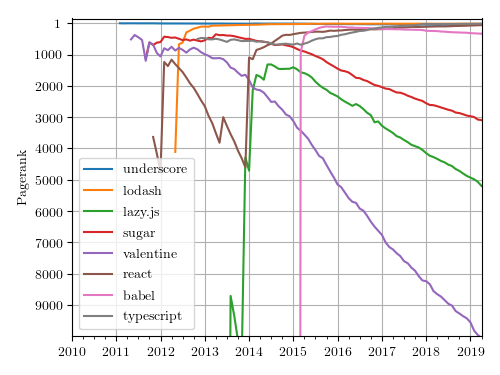
\includegraphics[width=0.5\textwidth]{figures/select_packages.png}
  \caption{\code{npm} rank (PageRank) over time of selected utility packages}
  \label{selectPackages}
\end{figure}

\section{Version Numbering and Package Adoption}
[NEEDS MORE DATA]

\subsection{Attribution of Version Numbers}
[NEEDS MORE DATA]

\subsection{Adoption by Version Number}
[NEEDS MORE DATA]

\section{Related Work}
[IN PROGRESS]


\section{Conclusion}
[NEEDS MORE DATA]


\begin{thebibliography}{10}

  \bibitem{Blincoe:2015}
  Kelly Blincoe, Francis Harrison, and Daniela Damian.
  \newblock Ecosystems in github and a method for ecosystem identification using
  reference coupling.
  \newblock In {\em Proceedings of the 12th Working Conference on Mining Software
  Repositories}, MSR '15, pages 202--207, Piscataway, NJ, USA, 2015. IEEE
  Press.

  \bibitem{brin1998anatomy}
  Sergey Brin and Lawrence Page.
  \newblock The anatomy of a large-scale hypertextual web search engine.
  \newblock {\em Computer networks and ISDN systems}, 30(1-7):107--117, 1998.

  \bibitem{DBLP:Decan:2018}
  Alexandre Decan, Tom Mens, and Philippe Grosjean.
  \newblock An empirical comparison of dependency network evolution in seven
  software packaging ecosystems.
  \newblock {\em CoRR}, abs/1710.04936, 2017.

  \bibitem{Gousi13}
  Georgios Gousios.
  \newblock The ghtorrent dataset and tool suite.
  \newblock In {\em Proceedings of the 10th Working Conference on Mining Software
  Repositories}, MSR '13, pages 233--236, Piscataway, NJ, USA, 2013. IEEE
  Press.

  \bibitem{Kikas:2017}
  Riivo Kikas, Georgios Gousios, Marlon Dumas, and Dietmar Pfahl.
  \newblock Structure and evolution of package dependency networks.
  \newblock In {\em Proceedings of the 14th International Conference on Mining
  Software Repositories}, MSR '17, pages 102--112, Piscataway, NJ, USA, 2017.
  IEEE Press.

  \bibitem{LUNGU2010264}
  Mircea Lungu, Michele Lanza, Tudor Gîrba, and Romain Robbes.
  \newblock The small project observatory: Visualizing software ecosystems.
  \newblock {\em Science of Computer Programming}, 75(4):264 -- 275, 2010.
  \newblock Experimental Software and Toolkits (EST 3): A special issue of the
  Workshop on Academic Software Development Tools and Techniques (WASDeTT
  2008).

  \bibitem{Manikas:2013}
  Konstantinos Manikas and Klaus~Marius Hansen.
  \newblock Software ecosystems - a systematic literature review.
  \newblock {\em J. Syst. Softw.}, 86(5):1294--1306, May 2013.

  \bibitem{Messerschmitt}
  David Messerschmitt and Clemens Szyperski.
  \newblock {\em Software Ecosystem: Understanding an Indispensable Technology
  and Industry}.
  \newblock 01 2003.

  \bibitem{Myers:2003}
  Christopher~R. Myers.
  \newblock Software systems as complex networks: Structure, function, and
  evolvability of software collaboration graphs.
  \newblock {\em Phys. Rev. E}, 68:046116, Oct 2003.

  \bibitem{DBLP:PanoGA16}
  Amantia Pano, Daniel Graziotin, and Pekka Abrahamsson.
  \newblock What leads developers towards the choice of a javascript framework?
  \newblock {\em CoRR}, abs/1605.04303, 2016.

  \bibitem{preston-werner}
  Tom Preston-Werner.
  \newblock Semantic versioning 2.0.0.

  \bibitem{Manikas:2017}
  M.~{Seppänen}, S.~{Hyrynsalmi}, K.~{Manikas}, and A.~{Suominen}.
  \newblock Yet another ecosystem literature review: 10+1 research communities.
  \newblock In {\em 2017 IEEE European Technology and Engineering Management
  Summit (E-TEMS)}, pages 1--8, Oct 2017.

  \bibitem{Serebrenik:2015}
  Alexander Serebrenik and Tom Mens.
  \newblock Challenges in software ecosystems research.
  \newblock In {\em Proceedings of the 2015 European Conference on Software
  Architecture Workshops}, ECSAW '15, pages 40:1--40:6, New York, NY, USA,
  2015. ACM.

  \bibitem{Wittern:2016}
  Erik Wittern, Philippe Suter, and Shriram Rajagopalan.
  \newblock A look at the dynamics of the javascript package ecosystem.
  \newblock In {\em Proceedings of the 13th International Conference on Mining
  Software Repositories}, MSR '16, pages 351--361, New York, NY, USA, 2016.
  ACM.

\end{thebibliography}

\vspace{12pt}

\end{document}
